%% ****** Start of file apstemplate.tex ****** %
%%
%%
%%   This file is part of the APS files in the REVTeX 4.2 distribution.
%%   Version 4.2a of REVTeX, January, 2015
%%
%%
%%   Copyright (c) 2015 The American Physical Society.
%%
%%   See the REVTeX 4 README file for restrictions and more information.
%%
%
% This is a template for producing manuscripts for use with REVTEX 4.2
% Copy this file to another name and then work on that file.
% That way, you always have this original template file to use.
%
% Group addresses by affiliation; use superscriptaddress for long
% author lists, or if there are many overlapping affiliations.
% For Phys. Rev. appearance, change preprint to twocolumn.
% Choose pra, prb, prc, prd, pre, prl, prstab, prstper, or rmp for journal
%  Add 'draft' option to mark overfull boxes with black boxes
%  Add 'showkeys' option to make keywords appear
%\documentclass[aps,prl,preprint,groupedaddress]{revtex4-2}
\documentclass[aps,prl,twocolumn,groupedaddress]{revtex4-2}
%\documentclass[aps,prl,preprint,superscriptaddress]{revtex4-2}
%\documentclass[aps,prl,reprint,groupedaddress]{revtex4-2}

% You should use BibTeX and apsrev.bst for references
% Choosing a journal automatically selects the correct APS
% BibTeX style file (bst file), so only uncomment the line
% below if necessary.
%\bibliographystyle{apsrev4-2}

\usepackage{graphicx}
\usepackage{subcaption}
\usepackage{caption}

\usepackage{epstopdf}
%\usepackage{amsmath}% http://ctan.org/pkg/amsmath
%\usepackage{amsthm}
%\usepackage{amsfonts}
%\usepackage{subfigure}
%\usepackage{hhline}
%\usepackage[miktex]{gnuplottex}
%\usepackage{xcolor}
\usepackage{amssymb}
\usepackage{amsmath}
\usepackage{color}
\usepackage{hyperref}
%\usepackage[percent]{overpic}
\usepackage{tikz}
\usepackage{mathrsfs}
\usepackage{wasysym}
\usepackage{tikz-cd}
%\usepackage{stix} %\fisheye
\usepackage{stackengine,scalerel}

% so sections, subsections, etc. become numerated.
\setcounter{secnumdepth}{3}

% Comandos proprios
\DeclareMathOperator*{\argmax}{arg\,max}
\DeclareMathOperator*{\argmin}{arg\,min}
\newcommand{\avrg}[1]{\left\langle #1 \right\rangle}
\newcommand{\nelta}{\bar{\delta}}
\newcommand{\bra}[1]{\left\langle #1\right|}
\newcommand{\ket}[1]{\left| #1 \right\rangle}
\newcommand{\sbra}[1]{\langle #1|}
\newcommand{\sket}[1]{| #1 \rangle}
\newcommand{\bek}[3]{\left\langle #1 \right| #2 \left| #3 \right\rangle}
\newcommand{\sbek}[3]{\langle #1 | #2 | #3 \rangle}
\newcommand{\braket}[2]{\left\langle #1 \middle| #2 \right\rangle}
\newcommand{\ketbra}[2]{\left| #1 \middle\rangle \middle\langle #2  \right|}
\newcommand{\sbraket}[2]{\langle #1 | #2 \rangle}
\newcommand{\sketbra}[2]{| #1 \rangle  \langle #2 |}
\newcommand{\norm}[1]{\left\lVert#1\right\rVert}
\newcommand{\snorm}[1]{\lVert#1\rVert}
\newcommand{\bvec}[1]{\boldsymbol{\mathsf{#1}}}
\newcommand{\bcov}[1]{\boldsymbol{#1}}
\newcommand{\bdua}[1]{\boldsymbol{\check{#1}}}
%\newcommand{\bdov}[1]{\boldsymbol{\breve{#1}}}
\newcommand{\bdov}[1]{\breve{#1}}
%\newcommand{\bten}[1]{\boldsymbol{\mathfrak{#1}}}
\newcommand{\bten}[1]{\boldsymbol{\mathfrak{#1}}}
\newcommand{\forany}{\tilde{\forall}}
\newcommand{\qed}{$\overset{\circ}{.}\;$}

\newcommand\bigeye{\ensurestackMath{\stackinset{c}{}{c}{-.3pt}%
  {\bullet}{\scriptstyle\bigcirc}}}
\newcommand\eye{\scalerel*{\bigeye}{x}}
%\newcommand*{\fisheye}{%
%    \mathbin{%
%        \ooalign{$\circledcirc$\cr\hidewidth$\bullet$\hidewidth}%
%    }%
%}
\renewcommand{\appendixname}{Apéndice} % Change "Appendix" to "Apéndice"

\begin{document}

% Use the \preprint command to place your local institutional report
% number in the upper righthand corner of the title page in preprint mode.
% Multiple \preprint commands are allowed.
% Use the 'preprintnumbers' class option to override journal defaults
% to display numbers if necessary
%\preprint{}

%Title of paper
\title{
Estudio del modelo de Hodgkin y Huxley
}

% repeat the \author .. \affiliation  etc. as needed
% \email, \thanks, \homepage, \altaffiliation all apply to the current
% author. Explanatory text should go in the []'s, actual e-mail
% address or url should go in the {}'s for \email and \homepage.
% Please use the appropriate macro foreach each type of information

% \affiliation command applies to all authors since the last
% \affiliation command. The \affiliation command should follow the
% other information
% \affiliation can be followed by \email, \homepage, \thanks as well.
\author{Luis Miguel Vargas Calderon}
\email[]{miguel.vargas@unc.edu.ar}
%\homepage[]{Your web page}
%\thanks{}
%\altaffiliation{}
%\affiliation{}
\affiliation{Facultad de Matem\'atica, Astronom\'ia, F\'isica y Computaci\'on, Universidad Nacional de C\'ordoba, Ciudad Universitaria, 5000 C\'ordoba, Argentina}

\author{Daniela Ruiz}
\email[]{danniela.vr31@gmail.com}
\affiliation{Facultad de Matem\'atica, Astronom\'ia, F\'isica y Computaci\'on, Universidad Nacional de C\'ordoba, Ciudad Universitaria, 5000 C\'ordoba, Argentina}



%Collaboration name if desired (requires use of superscriptaddress
%option in \documentclass). \noaffiliation is required (may also be
%used with the \author command).
%\collaboration can be followed by \email, \homepage, \thanks as well.
%\collaboration{Juan Perez}
%\noaffiliation

\date{\today}

\begin{abstract}
El objetivo de este trabajo es estudiar el comportamiento del modelo de Hodgkin-Huxley, utilizando métodos de integración numérica.
\end{abstract}

% insert suggested keywords - APS authors don't need to do this
%\keywords{}

%\maketitle must follow title, authors, abstract, and keywords
\maketitle

\section{Introducción}

El modelo de Hodgkin y Huxley describe cómo se inician y transmiten los potenciales de acción en las neuronas.

Consiste en un conjunto de cuatro ecuaciones diferenciales ordinarias acopladas no lineales, que aproximan las características eléctricas de células excitables como las neuronas.
~\cite{hertz1999introduction}.

\section{Teoría}

Las siguientes ecuaciones diferenciales
detalladas en ~\cite{hertz1999introduction}
son las  que modelan el comportamiento del potencial de las neuronas cuando son ejercitadas con inpulsos de iones.

\begin{eqnarray*}
\dot{n}&=&\alpha_n(v)(1-n)-\beta_n(v) n\\
\dot{m}&=&\alpha_m(v)(1-m)-\beta_m(v) m\\
\dot{h}&=&\alpha_h(v)(1-h)-\beta_h(v) h\\
\dot{v}&=&c^{-1}(i-\bar{g}_{\mathrm{Na}}m^3h(v-v_{\mathrm{Na}})-\bar{g}_{\mathrm{K}}n^4(v-v_{\mathrm{K}})-g_{l}(v-v_{l}))
\end{eqnarray*}

Utilizando el metodo de integracon de Runge Kutta se logra aproximar COMPLETAR o MEJORAR



Se definieron varias funciones que modelan el impuslo de corriente
 denominadas como i, i2, etc

 la fucncion de integracion toma como parametros las ecuaciones diferenciasles que a su vez en cada expermiento estan parametrizadas por cada una de las funciones de corrientes
 Se realizaron 5 experimentos.
 
COMPLETAR o MEJORAR

\section{Resultados}

Experimento 1) Se utilizo una funcon de corriente que devuelve la constante 0. MODELAR O COMPLETAR.
El potencial de la membrana modelado muestra que:
 MODELAR O COMPLETAR. Ver fig.~\ref{fig1}.

\begin{figure}[h!]
\centering
\begin {subfigure}{0.45\textwidth}
\centering
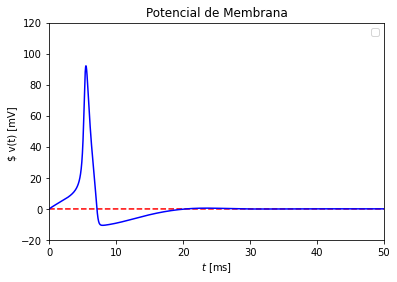
\includegraphics [width=1\textwidth]{figs/potencial_de_membrana.png}
\caption{zaraza}
\label{fig1}
\end{subfigure}\\

\begin {subfigure} {0.45\textwidth}
\centering
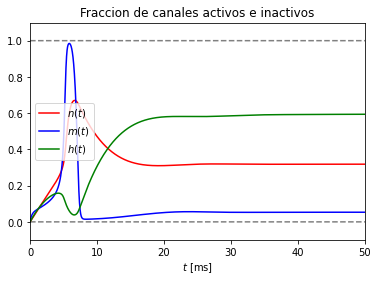
\includegraphics [width=1\textwidth] {figs/fraccion_de_canales_activos_e_inactivos}
\caption{zaraza2}
\end{subfigure}
\caption{zaraza3}
\label{fig1}
\end{figure}


Experimento 2) Se utilizo una funcon de orriente que devuelve la constante 0. MODELAR O COMPLETAR.

El potencial de la membrana modelado muestra que:
 MODELAR O COMPLETAR.

Ver fig.~\ref{fig2}.

\begin{figure}[h!]
\centering
\begin {subfigure}{0.45\textwidth}
\centering
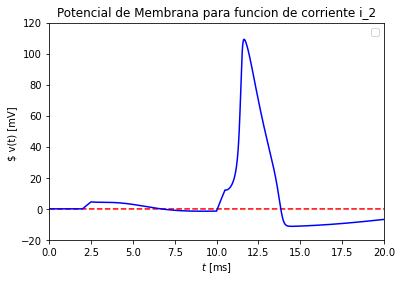
\includegraphics [width=1\textwidth]{figs/potencial_membrana_i_2.png}
\caption{zaraza}
\label{fig1}
\end{subfigure}\\

\begin {subfigure} {0.45\textwidth}
\centering
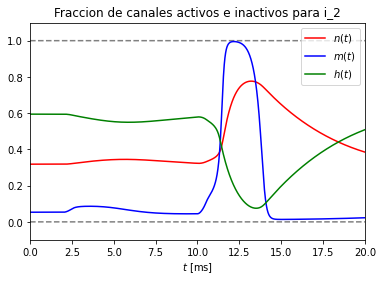
\includegraphics [width=1\textwidth] {figs/fraccion_de_canales_activos_e_inactivos_para_i_2.png}
\caption{zaraza2}
\end{subfigure}
\caption{zaraza3}
\label{fig1}
\end{figure}



Experimento 3) Se utilizo una funcon de corriente que devuelve la constante 0. MODELAR O COMPLETAR.

El potencial de la membra
Ver fig.~\ref{fig3}.
\begin{figure}[h!]
\centering
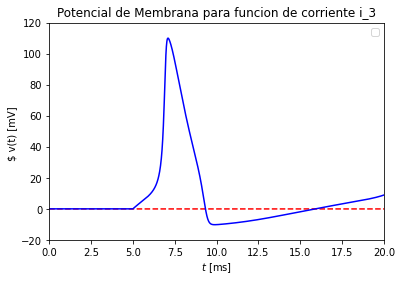
\includegraphics[scale=.4]{figs/potencial_membrana_i_3.png}
%\vspace{-0.25cm}
\caption{
Potencial de membrana función i3. \label{fig3}
}
\end{figure}

Experimento 4) Se utilizo una funcon de orriente que devuelve la constante 0. MODELAR O COMPLETAR.

El potencial de la membra
Ver fig.~\ref{fig4}.

\begin{figure}[h!]
\centering
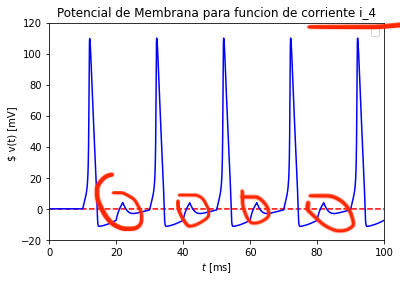
\includegraphics[scale=.4]{figs/potencial_membrana_i_4.png}
%\vspace{-0.25cm}
\caption{
Potencial de membrana función i4.\label{fig4}
}
\end{figure}

Experimento ) Se utilizo una funcon de orriente que devuelve la constante 0. MODELAR O COMPLETAR.

El potencial de la membra
Ver fig.~\ref{fig5}.

\begin{figure}[h!]
\centering
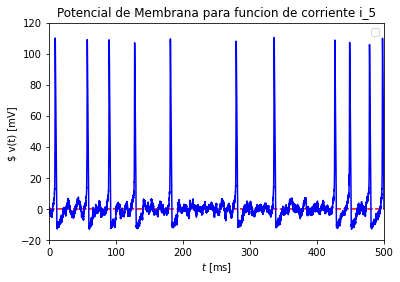
\includegraphics[scale=.35]{figs/potencial_membrana_i_5.png}
%\vspace{-0.25cm}
\caption{
Potencial de membrana función i5. \label{fig5}
}
\end{figure}









\section{Discusión}

La comparación de ................................................................
...............................................................
.. bla bla bla ................................................................
...............................................................
.. bla bla bla

\section{Conclusiones}

Concluyendo ................................................................
........................................................

% If in two-column mode, this environment will change to single-column
% format so that long equations can be displayed. Use
% sparingly.
%\begin{widetext}
% put long equation here
%\end{widetext}

% figures should be put into the text as floats.
% Use the graphics or graphicx packages (distributed with LaTeX2e)
% and the \includegraphics macro defined in those packages.
% See the LaTeX Graphics Companion by Michel Goosens, Sebastian Rahtz,
% and Frank Mittelbach for instance.
%
% Here is an example of the general form of a figure:
% Fill in the caption in the braces of the \caption{} command. Put the label
% that you will use with \ref{} command in the braces of the \label{} command.
% Use the figure* environment if the figure should span across the
% entire page. There is no need to do explicit centering.

% \begin{figure}
% \includegraphics{}%
% \caption{\label{}}
% \end{figure}

% Surround figure environment with turnpage environment for landscape
% figure
% \begin{turnpage}
% \begin{figure}
% \includegraphics{}%
% \caption{\label{}}
% \end{figure}
% \end{turnpage}

% tables should appear as floats within the text
%
% Here is an example of the general form of a table:
% Fill in the caption in the braces of the \caption{} command. Put the label
% that you will use with \ref{} command in the braces of the \label{} command.
% Insert the column specifiers (l, r, c, d, etc.) in the empty braces of the
% \begin{tabular}{} command.
% The ruledtabular enviroment adds doubled rules to table and sets a
% reasonable default table settings.
% Use the table* environment to get a full-width table in two-column
% Add \usepackage{longtable} and the longtable (or longtable*}
% environment for nicely formatted long tables. Or use the the [H]
% placement option to break a long table (with less control than 
% in longtable).
% \begin{table}%[H] add [H] placement to break table across pages
% \caption{\label{}}
% \begin{ruledtabular}
% \begin{tabular}{}
% Lines of table here ending with \\
% \end{tabular}
% \end{ruledtabular}
% \end{table}

% Surround table environment with turnpage environment for landscape
% table
% \begin{turnpage}
% \begin{table}
% \caption{\label{}}
% \begin{ruledtabular}
% \begin{tabular}{}
% \end{tabular}
% \end{ruledtabular}
% \end{table}
% \end{turnpage}

%\section{Aknowledgments}
\section{Agradecimientos}

\begin{acknowledgments}
JIP, BM y MA agradecen el finaciamiento y el apoyo de CONICET, SeCyT y la UNC.
\end{acknowledgments}
% Create the reference section using BibTeX:
\bibliography{ref}

% Specify following sections are appendices. Use \appendix* if there
% only one appendix.

\onecolumngrid

\appendix

Bla bla bla...

\end{document}
%
% ****** End of file apstemplate.tex ******


